\newpage
\section{Procedures}

To setup a comfortable workflow for developing ROS packages, also for the sake of the simplicity of developling environment, and most importantly, let the simulation run smoothly on my old laptop, the instructions on how to install and configure Oracle VM VirtualBox, Ubuntu with desktop environment, CLion, and ros-noetic-desktop-full Debian package were not followed. Instead, ros:noetic Docker container, VcXsrv X server, and VSCode with container development extension were used. In addition, GCC which is default C/C++ complier for Linux were replaced by Clang-12. To have syntanx highlight in VSCode, Clangd-12 language server and two extensions, Clangd and CMake Tools, were installed.

\begin{figure}[htbp]
   \centering
   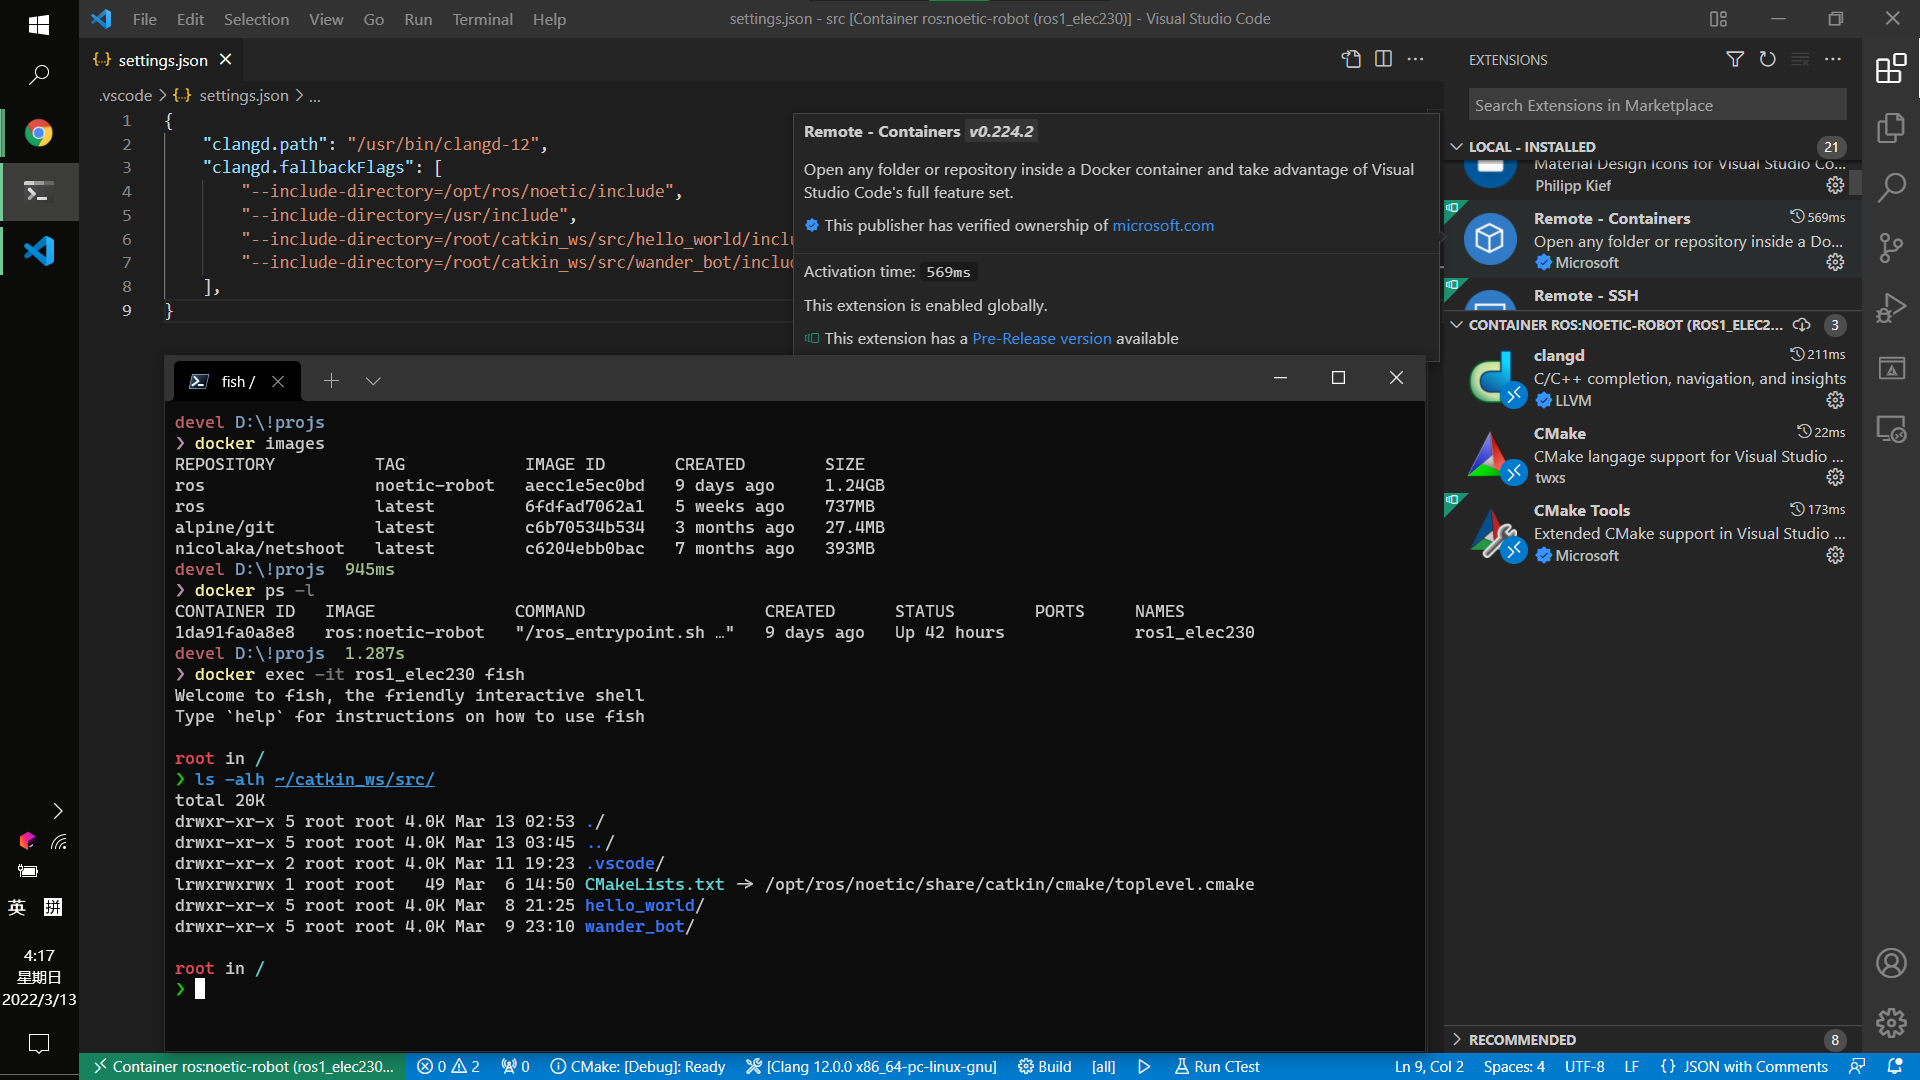
\includegraphics[width=0.9\textwidth]{figures/devel_env.png}
   \caption{Develop environment}
   \label{fig:devel_env}
\end{figure}

The assignment requires using Catkin build system. To work with it, first create a folder for Catkin Workspace in home directory and another in it which holds source files. Then using command
\begin{minted}[fontsize=\footnotesize, breaklines]{shell-session}
root@ROS1:~/catkin_ws/src$ catkin_create_pkg wander_bot roscpp rospy std_msgs
\end{minted}
to create a package with three dependencies which will later be delivered to assignment assessor via Canvas.

To speed up the workflow in the terminal, the shell was changed from bash to fish, and fish was configured to automatically source ROS1 and Catkin Workspace according to the instructions on the ROS1 wiki rosbash page \cite{ref:rosbash}.

The developing process was a simple cycle: modify the code, observe the simulation, modify the code... After the simulation works as expected, the code was cleaned, the file sturcture was re-orgnaised, and the code comments was enriched.

\section{Results}

The program was executed as per the procedure specified in the assignment manual \cite{ref:ass3_manual}. See figure \ref{fig:source_install_and_execute}.

\begin{figure}[htbp]
   \centering
   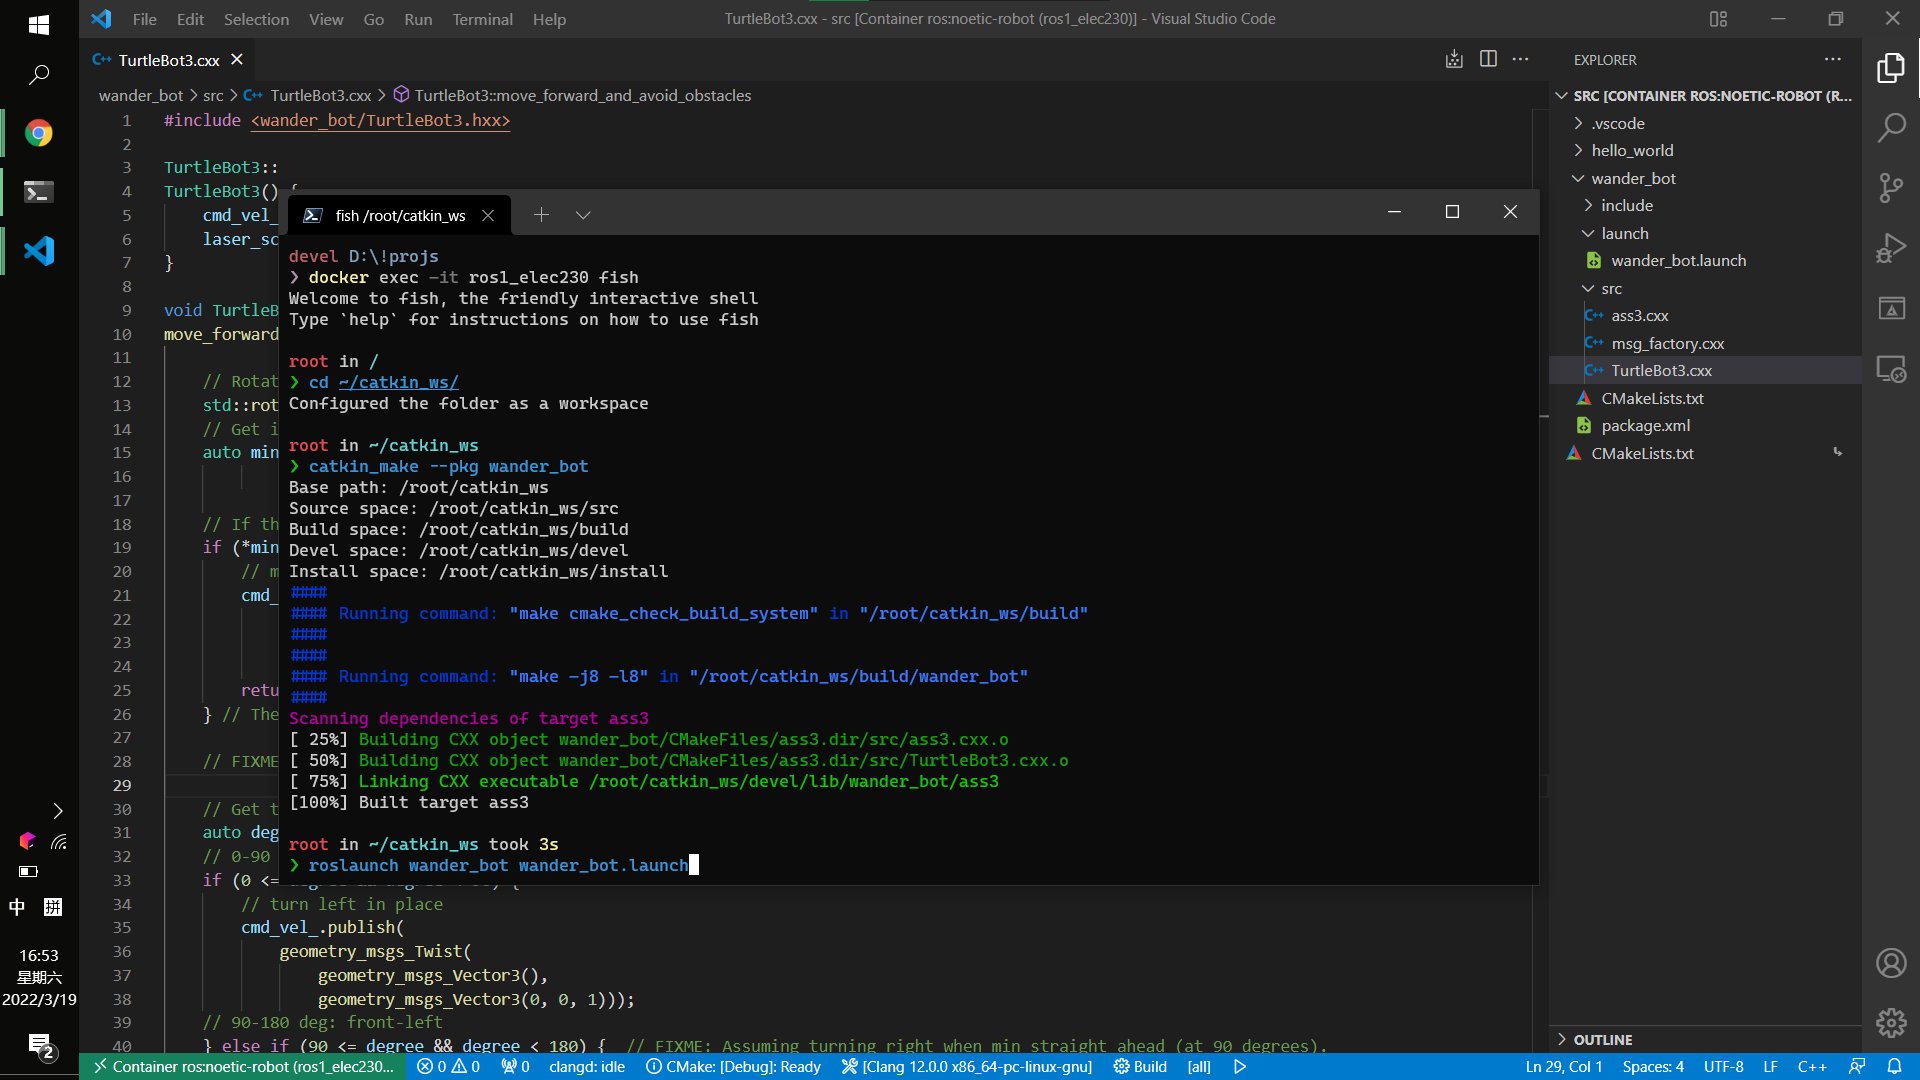
\includegraphics[width=0.9\textwidth]{figures/source_install_and_execute.png}
   \caption{Sourcing, installing, and executing}
   \label{fig:source_install_and_execute}
\end{figure}

The simulation environment was opened, the node for controlling the robot started, as shown in Figure \ref{fig:sim_started}. Then, the robot started transmitting laser scan data to the node which processes the data according to the algorithm and sends a message instructing the robot to move.

\begin{figure}[htbp]
   \centering
   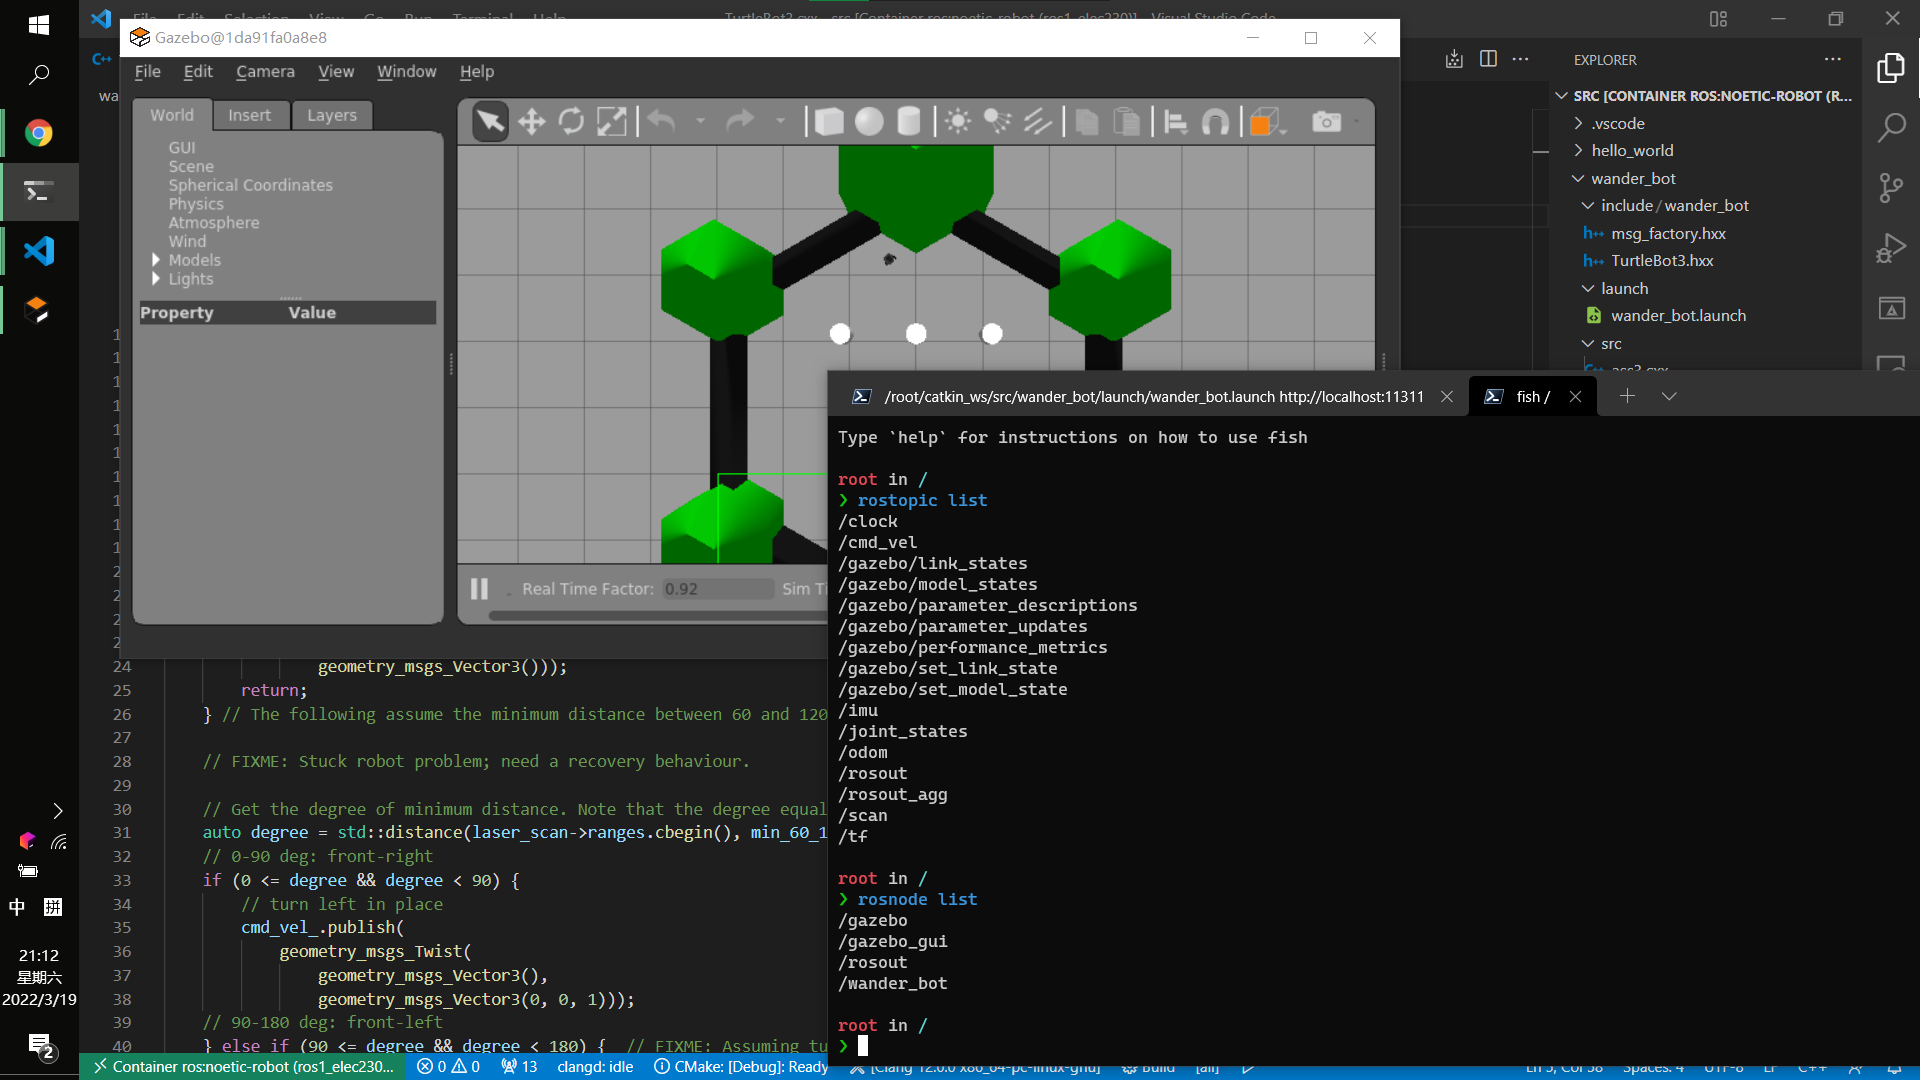
\includegraphics[width=0.9\textwidth]{figures/sim_started.png}
   \caption{Simulation started}
   \label{fig:sim_started}
\end{figure}

\section{Testing}

Set linear velocity to 0.3 m/s, angular velocity to 1 rad/s, TurtleBot3 could successfully avoid regular obstacles for at least ten minutes.

\begin{figure}[htbp]
   \centering
   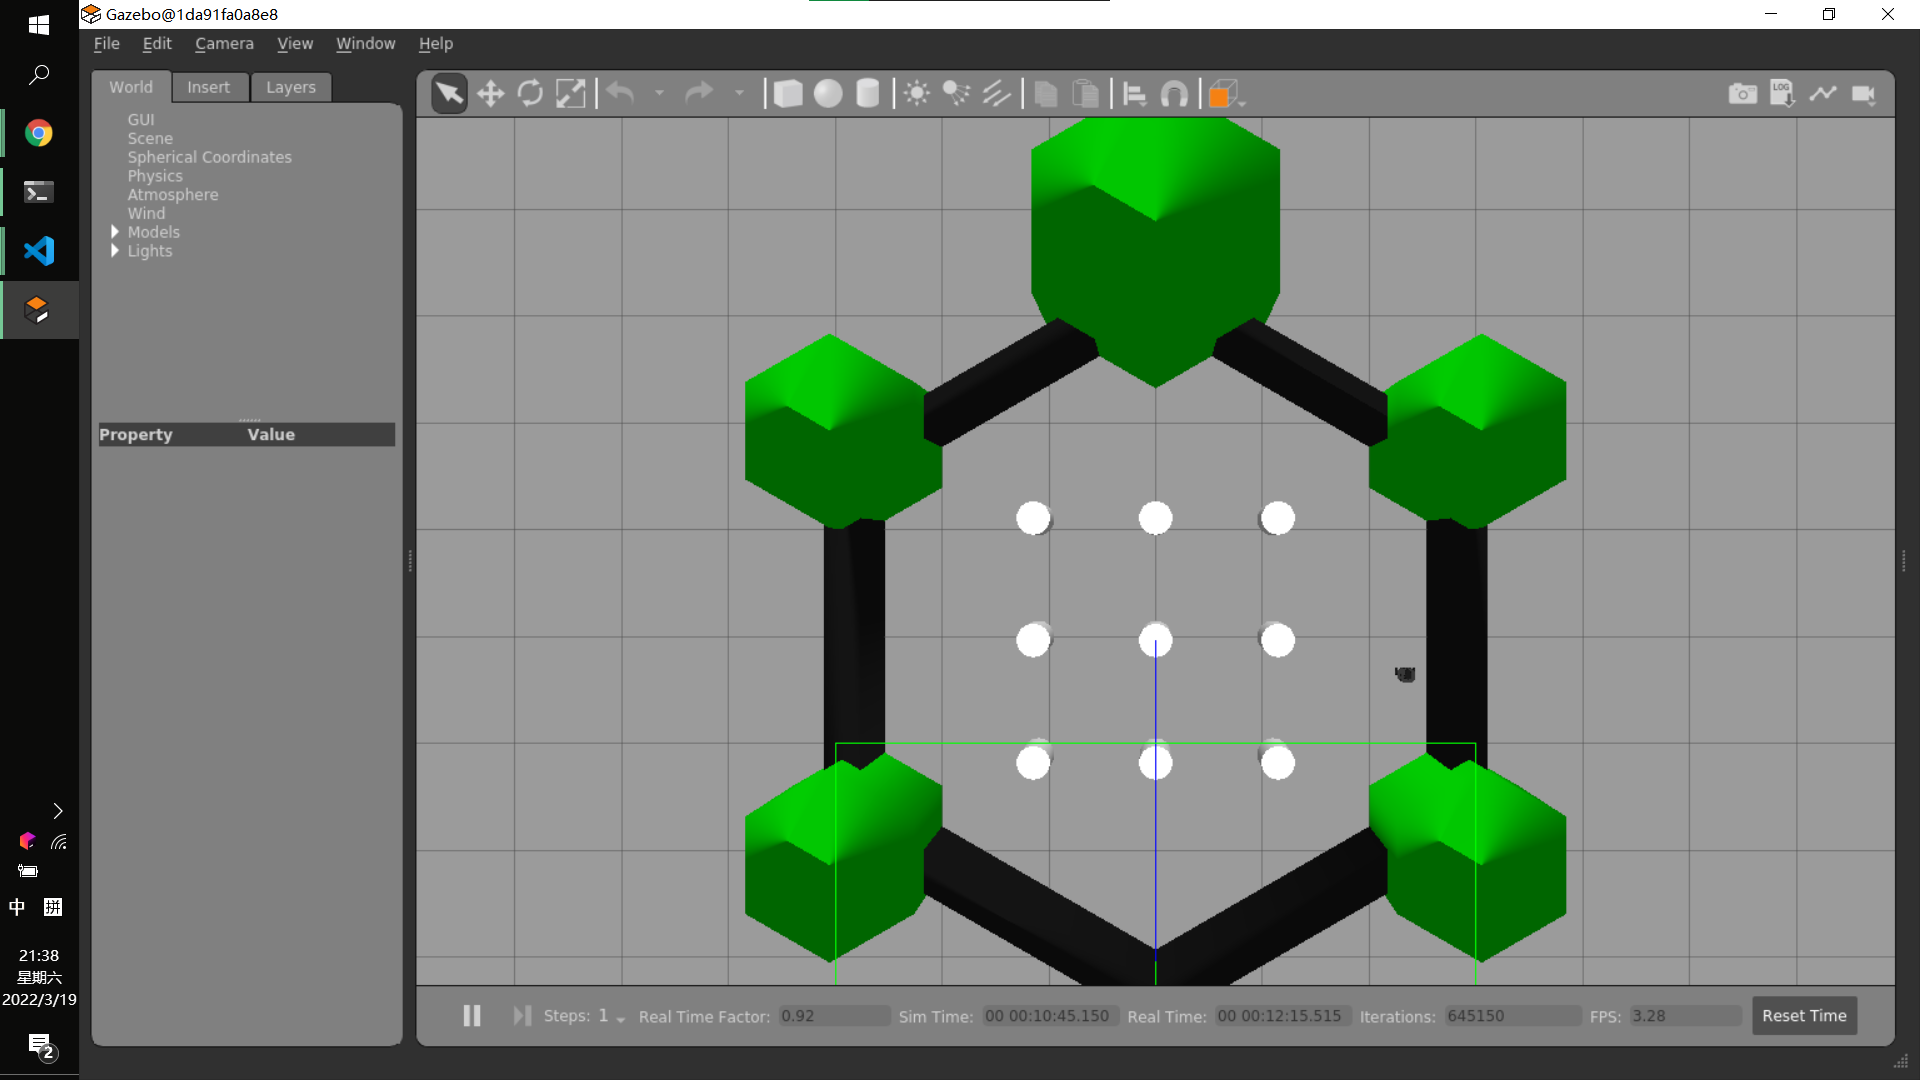
\includegraphics[width=0.9\textwidth]{figures/test_10min.png}
   \caption{Avoiding regular obstacles with moderate velocities for about ten minutes}
   \label{fig:test_10min}
\end{figure}

When the linear velocity was increased to 1 m/s, the robot would not have time to react and would hit the obstacle. Once it hitted the obstacle, the robot was likely to get stuck and unable to rotate as shown in Figure \ref{fig:test_high_linear_vel}.

\begin{figure}[htbp]
   \centering
   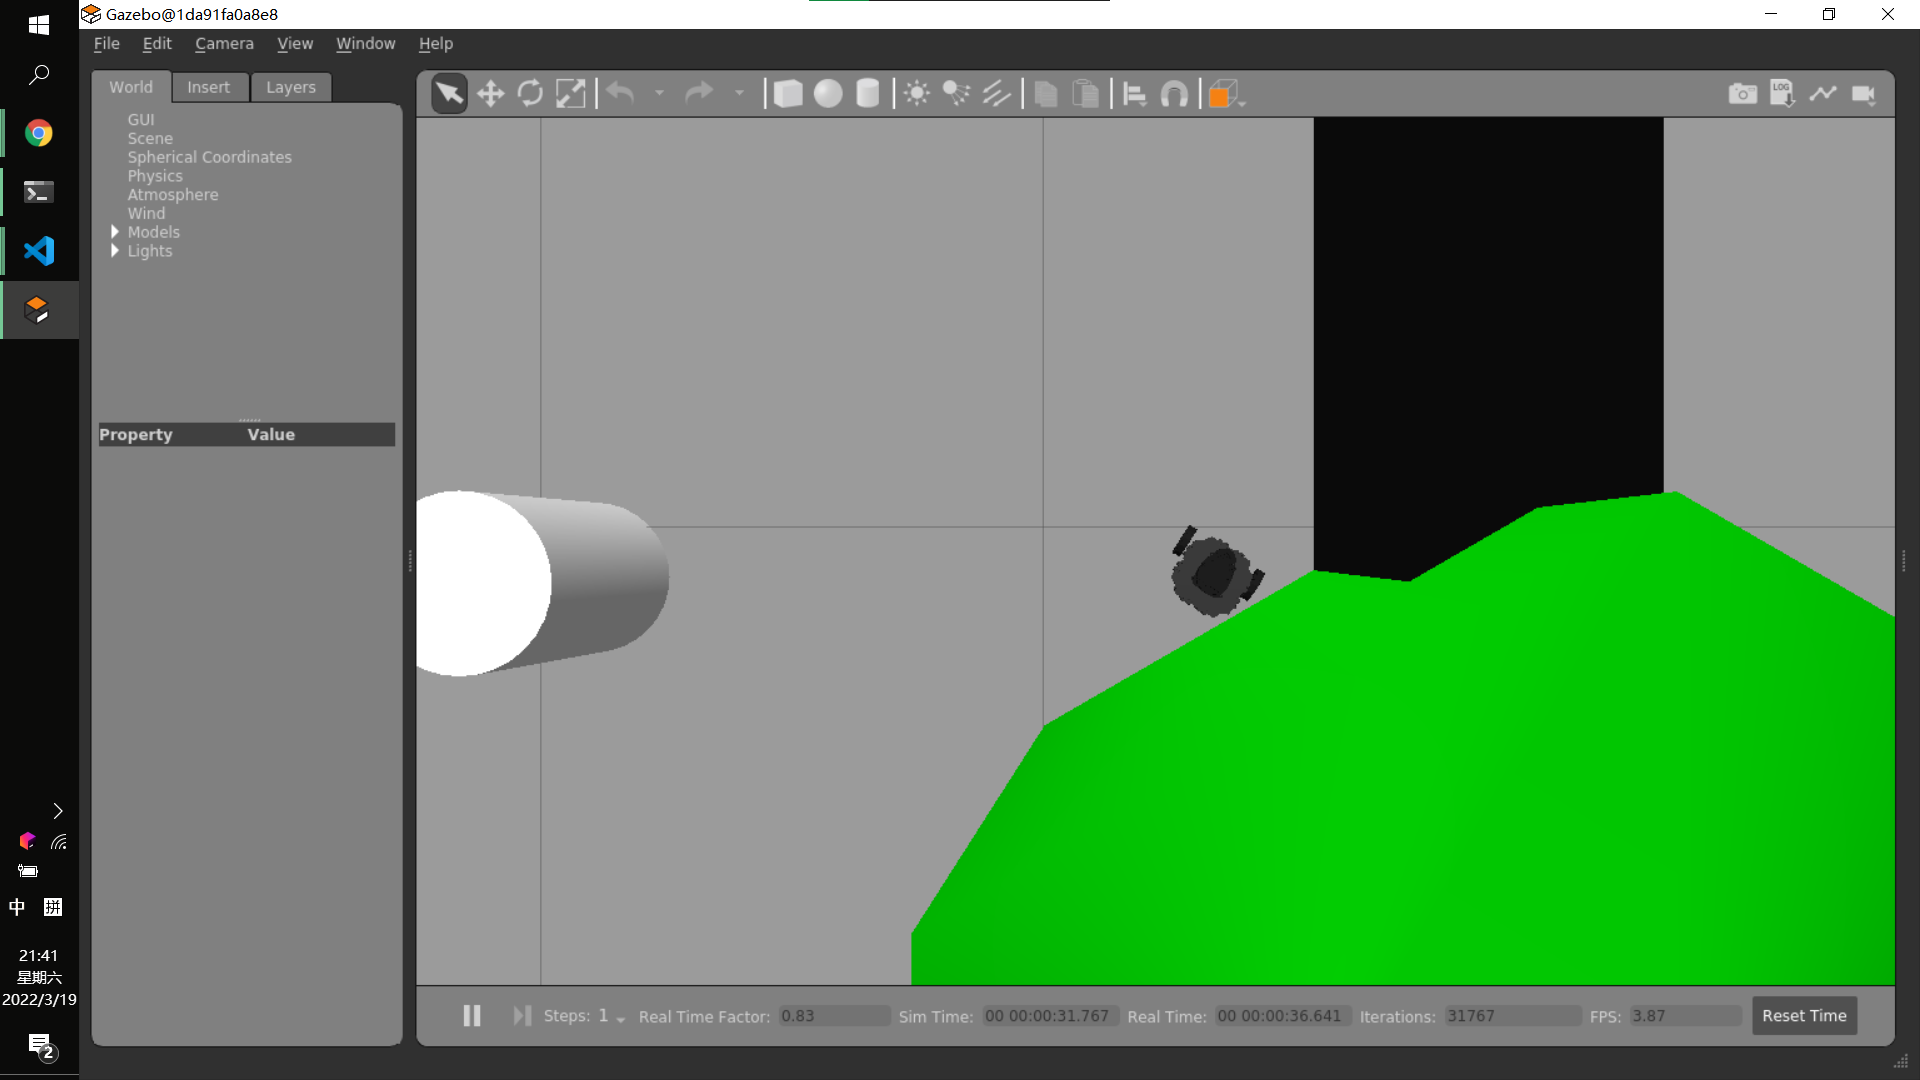
\includegraphics[width=0.9\textwidth]{figures/test_high_linear_vel.png}
   \caption{TurtleBot3 hits the wall and then gets stuck and can't rotate}
   \label{fig:test_high_linear_vel}
\end{figure}

Figure \ref{fig:test_corner} demonstrates that the robot can also get stuck when it encounters sharp corners.

\begin{figure}[htbp]
   \centering
   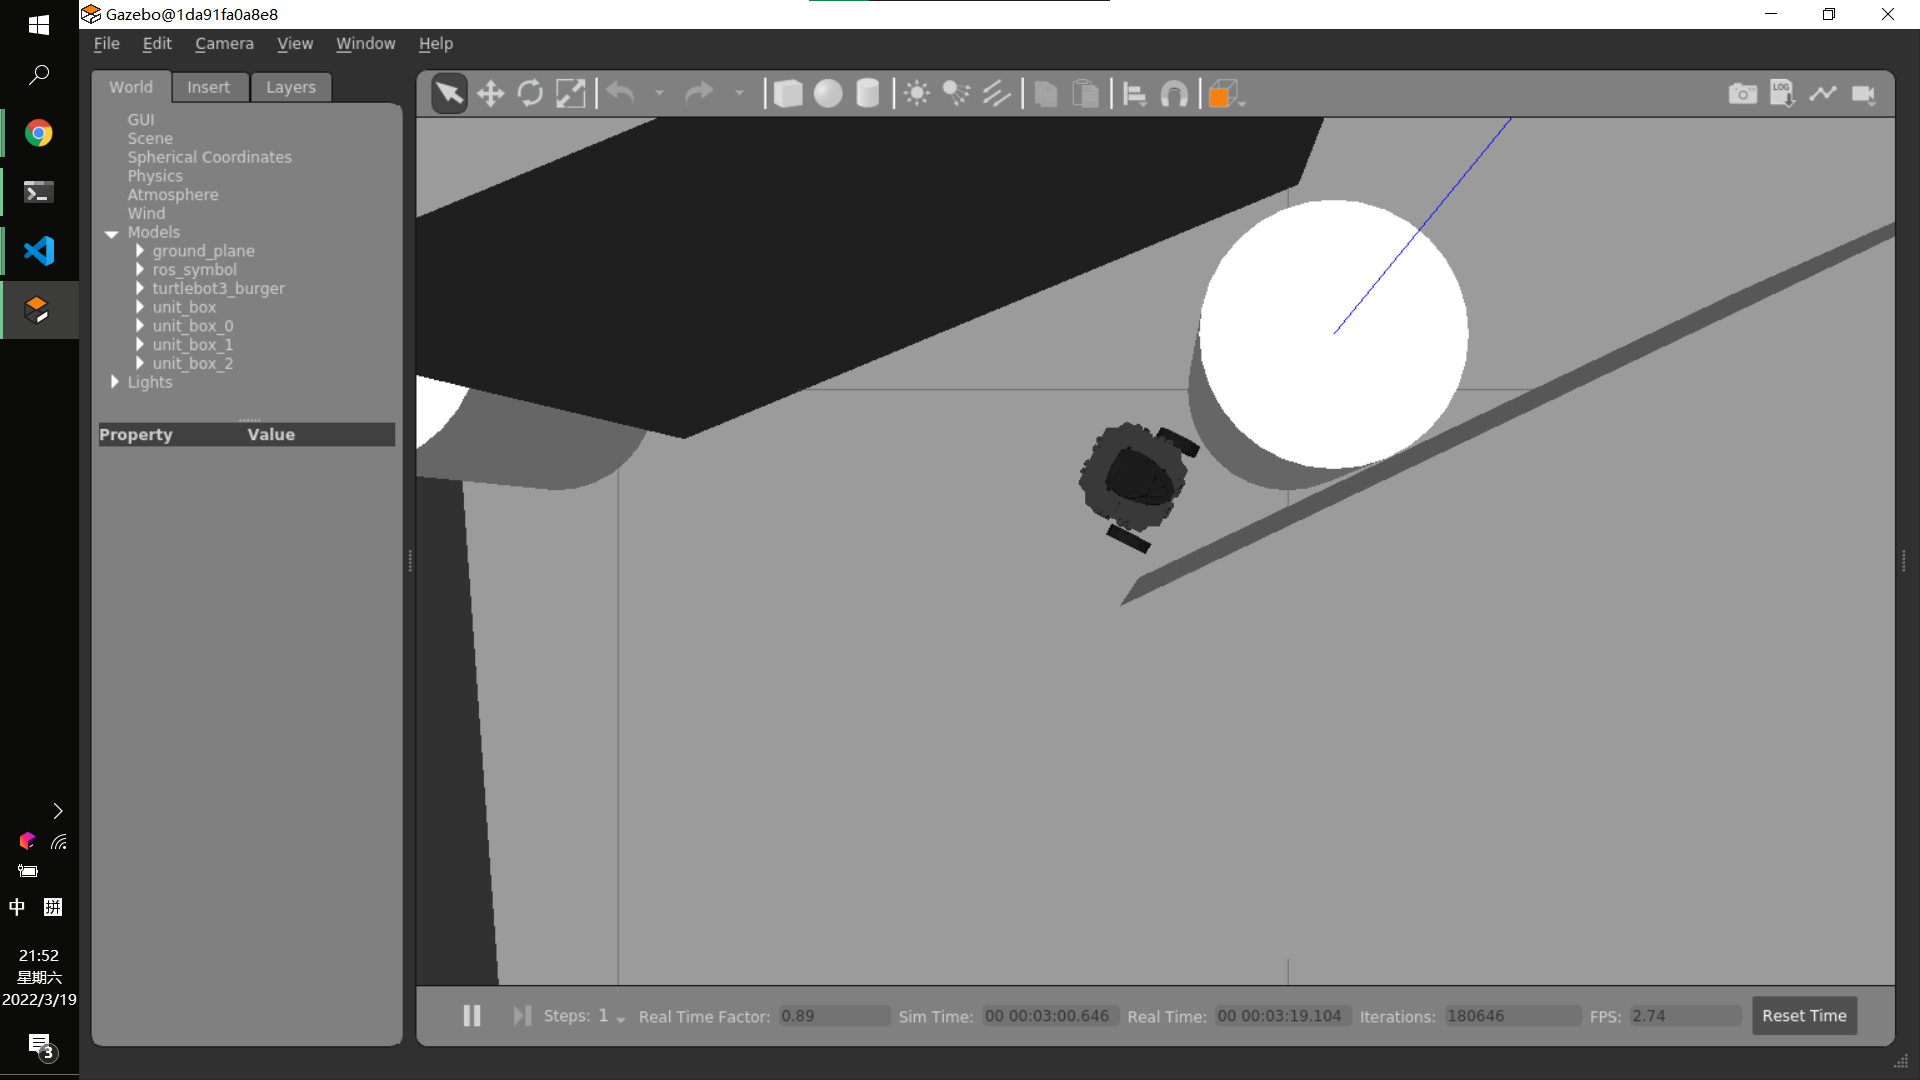
\includegraphics[width=0.8\textwidth]{figures/test_corner.png}
   \caption{TurtleBot3 swinging in a sharp corner}
   \label{fig:test_corner}
\end{figure} 

\section{What worked and what did not}

With regular obstacles, the algorithm is able to turn right with the obstacle on the left and left with the obstacle on the right. However, it is likely that the behaviour when encountering an irregular obstacle will not be as expected, as the algorithm only takes into account the minimum value of one angle of the laser scan.

In the course of writing the code it was found that controlling linear and angular velocity seperately in a concise way is difficult because they are warpped in a single data structure, geometry\_msgs::Twist, and the TurtleBot3's controller did not honor "ignore NaN" convention; TurtleBot3 moves backward after receiving NaN. This results in logic that should be separated in the algorithm not being separated, which might against the Don't Repeat Yourself principle if the program was developed further.

The maximum frequency of spin is set in the main function by ros::Rate rate(10), but the publishing frequency of the data from the laser scan is much lower than 10Hz. If the angular velocity is set fast but the laser scan sends data slowly, the robot may oversteer, since it is velocity controlled.

The algorithm does not allow the robot to follow the wall when it encounters it, but it is a necessary behaviour for the robot vacuum cleaner.
